\documentclass[12pt]{amsart}
\usepackage{graphicx} % Required for inserting images
\usepackage{amsthm}
\usepackage{amsmath}
\usepackage{amssymb}
\usepackage{hyperref}
\usepackage{tikz}
\usetikzlibrary{arrows.meta, calc, positioning}

\theoremstyle{plain}
\newtheorem{theorem}{Theorem}[section]
\newtheorem{proposition}{Proposition}[section]
\newtheorem{lemma}{Lemma}[section]
\newtheorem{corollary}{Corollary}[section]

\theoremstyle{definition}
\newtheorem{definition}{Definition}[section]
\newtheorem{example}{Example}[section]
\newtheorem{construction}{Construction}[section]

\theoremstyle{remark}
\newtheorem{remark}{Remark}[section]
\newtheorem{note}{Note}[section]

\newcommand{\R}{\mathbb{R}}
\newcommand{\A}{\mathcal{A}}
\newcommand{\V}{\mathcal{V}}

\title{Hyperplane Arrangements and Combinatorial Complexity}
\author{Siddharth Krishna}

\begin{document}

\begin{abstract}
This paper presents an introduction to the combinatorial and geometric structure of real hyperplane arrangements. We develop the notions of regions, faces, and sign patterns, and introduce the intersection poset and characteristic polynomial. Zaslavsky's theorem is stated and illustrated through computations in low dimensions. We then describe the face poset and oriented sign-vector structure, which together encode the stratification of space induced by an arrangement. Finally, we connect these ideas to piecewise-linear functions, specifically a single-layer ReLU network, which defines a hyperplane arrangement whose regions correspond to the layer's linear pieces, and whose structure reflects aspects of expressiveness and fragility.
\end{abstract}

\maketitle

\section{Introduction}
A finite collection of hyperplanes in a real vector space partitions the space into convex regions, and the way these regions intersect encodes combinatorial structure. For instance, in $\R^2$ two nonparallel lines divide the plane into four regions, while three lines in general position divide it into seven. Understanding why such numbers arise, and how they change as hyperplanes move or are added, is a central theme in the study of arrangements.

This perspective forms the basis for tools such as the intersection poset and the characteristic polynomial. Hyperplane arrangements can help reduce geometric questions to purely combinatorial ones. For example, the number of connected regions determined by an arrangement depends only on the poset of its intersections, and Zaslavsky’s theorem expresses this number in terms of the M\"obius function of that poset. Understanding how regions fit together leads naturally to the face poset and oriented sign structures, which encode adjacency and orientation information.

These concepts are also relevant in studying piecewise-linear models in machine learning. A feedforward neural network with ReLU activations implements a function that is linear on each region of a hyperplane arrangement defined by its activation boundaries. The expressive behavior and local sensitivity of such models can be viewed through the geometry and combinatorics of these arrangements.

\section{Preliminaries}
\noindent First, we recall the basic definitions and examples needed to study hyperplane arrangements.

\begin{definition}[Affine hyperplane]
An \emph{affine hyperplane} in $\R^d$ is a set of the form
\[
H = \{ x \in \R^d : w \cdot x + b = 0 \},
\]
where $w \in \R^d$ is a nonzero vector and $b \in \R$.
The hyperplane divides $\R^d$ into the open half-spaces
\[
H^{+} = \{x : w \cdot x + b > 0\}, \qquad
H^{-} = \{x : w \cdot x + b < 0\}.
\]
\end{definition}

\begin{definition}[Hyperplane arrangement]
A \emph{hyperplane arrangement} in $\R^d$ is a finite collection
\[
\A = \{H_1, \dots, H_n\}
\]
of affine hyperplanes.  
The \emph{complement} of $\A$ is
\[
M(\A) = \R^d \setminus \bigcup_{i=1}^n H_i.
\]
The connected components of $M(\A)$ are the \emph{regions}
of the arrangement.  
We denote by $R(\A)$ the set of regions, and by
\[
r(\A) = \# R(\A)
\]
the number of regions.
\end{definition}

\begin{definition}[Sign pattern]
Given an arrangement $\A = \{H_1,\dots,H_n\}$ with defining
forms $w_i \cdot x + b_i$, the \emph{sign pattern} of a point
$x \in \R^d$ is the vector
\[
\sigma(x) = 
(\operatorname{sign}(w_1 \cdot x + b_1),\dots,
 \operatorname{sign}(w_n \cdot x + b_n))
\in \{-,0,+\}^n.
\]
\end{definition}

\begin{proposition}
Two points $x,y \in \R^d$ lie in the same region of $\A$ iff
\[
\operatorname{sign}(w_i \cdot x + b_i)
  = \operatorname{sign}(w_i \cdot y + b_i)
  \qquad \text{for all } i.
\]
Thus, each region corresponds to a unique sign pattern of the linear forms
$\{ w_i \cdot x + b_i \}$. In particular, the sign map $\sigma\colon \R^d \to \{-,0,+\}^n$ is locally constant on each region.
\end{proposition}

\begin{proof}[Idea of proof]
If two points lie in the same region, then any path between them avoids all hyperplanes, so none of the values $w_i \cdot x + b_i$ can change sign.  
Conversely, if all signs agree, one can move from $x$ to $y$ while  remaining on the same side of every hyperplane, so no hyperplane is crossed; hence $x$ and $y$ lie in the same region.
\end{proof}

\begin{definition}[Flat and intersection poset]
Given a subcollection of hyperplanes $H_{i_1}, \dots, H_{i_k}$, their intersection
\[
X = H_{i_1} \cap \cdots \cap H_{i_k}
\]
is called a \emph{flat}.  
The set of all nonempty flats, together with $\R^d$, ordered by reverse inclusion
\[
X \le Y \quad \iff \quad Y \subseteq X,
\]
forms the \emph{intersection poset} of the arrangement.
\end{definition}

\begin{definition}[Face]
A \emph{face} of $\A$ is any nonempty set obtained by choosing, for each hyperplane $H_i$, one of the conditions
\[
w_i \cdot x + b_i > 0, \qquad
w_i \cdot x + b_i = 0, \qquad
w_i \cdot x + b_i < 0,
\]
whenever the resulting set is nonempty.  
A region is a top-dimensional face (all strict inequalities).
Lower-dimensional faces lie on the hyperplanes themselves.
\end{definition}

Here are a few examples in low dimensions:

\begin{example}[Two lines in $\R^2$]
Two nonparallel lines intersect in one point and divide the plane into four regions. Each region corresponds to a distinct sign pattern for the two defining linear forms.
\end{example}

\begin{figure}[h]
\centering
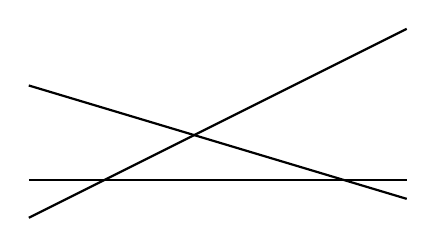
\begin{tikzpicture}[scale=1.2]
  % three lines in general position (no two parallel, no triple intersection)
  \draw[thick] (-2,0) -- (2,0);           % horizontal
  \draw[thick] (-2,-0.4) -- (2,1.6);      % up-sloping
  \draw[thick] (-2,1.0) -- (2,-0.2);      % down-sloping

  % optionally, mark one region lightly (comment out if you don't want it)
  %\fill[gray!15] (0,0) -- (1,0) -- (1,0.6) -- (0,0.4) -- cycle;
\end{tikzpicture}
\caption{Three lines in general position in $\mathbb R^2$ forming seven regions.}
\label{fig:three-lines}
\end{figure}

\begin{example}[Three lines in general position]
Three pairwise nonparallel lines form three intersection points and partition $\R^2$ into seven regions; see Figure~\ref{fig:three-lines}.  
This illustrates that region counts depend on the intersections, not just on the number of hyperplanes.
\end{example}

\begin{example}[Three planes in $\R^3$]
Three planes in general position intersect in a single point and divide space into eight regions, the three-dimensional analogue of the quadrants in $\R^3$.
\end{example}

\section{The Characteristic Polynomial and Zaslavsky's Theorem}
In this section we introduce the characteristic polynomial of a hyperplane arrangement and state Zaslavsky's theorem, which expresses the number of regions of an arrangement in terms of this polynomial.

\begin{definition}[M\"obius function]
Let $L(\A)$ be the intersection poset of an arrangement $\A$, ordered by reverse inclusion. The M\"obius function $\mu$ of $L(\A)$ is defined recursively by
\[
\mu(X,X)=1 \qquad\text{for all } X\in L(\A),
\]
and for $X<Y$,
\[
\sum_{X \le Z \le Y} \mu(X,Z)=0.
\]
\end{definition}

\begin{definition}[Characteristic polynomial]
The \emph{characteristic polynomial} of the arrangement $\A$ is
\[
\chi_{\A}(t)=\sum_{X\in L(\A)} \mu(\R^d,X)\, t^{\dim(X)}
\]
(see \cite{ChenWang}.)
\end{definition}

The characteristic polynomial can be computed directly from the intersection poset, and its coefficients encode information about the combinatorics of the arrangement. The appearance of the M\"obius function reflects an inclusion-exclusion principle on the poset: the values $\mu(\R^d,X)$ play the role of alternating weights that correct for overcounting when summing contributions from different hyperplane intersections. In particular, $\chi_{\A}(t)$ depends only on the structure of $L(\A)$ and the M\"obius function.

\begin{example}
For two nonparallel lines in $\R^2$, the poset consists of $\R^2$, the two lines, and their intersection point. Performing the computation gives
\[
\chi_{\A}(t)=t^2-2t+1.
\]
Evaluating at $t=-1$ yields $\chi_{\A}(-1)=4$, which matches the four regions determined by the two lines.
\end{example}

\begin{example}
Three lines in general position in $\R^2$ have intersection poset consisting of the plane, the three lines, and the three intersection points. We find that
\[
\chi_{\A}(t)=t^2-3t+3.
\]
Evaluating at $t=-1$ gives $\chi_{\A}(-1)=7$.
\end{example}

\begin{definition}[Rank]
Let $\A$ be an arrangement in $\R^d$ with hyperplanes
\[
H_i = \{ x \in \R^d : w_i \cdot x + b_i = 0 \}.
\]
The \emph{rank} of $\A$ is
\[
\mathrm{rank}(\A) = \dim \operatorname{span}\{w_1,\dots,w_n\}.
\]
It measures the effective dimension in which the arrangement cuts space.
\end{definition}

Zaslavsky's theorem expresses the number of regions and bounded regions of a real arrangement purely in terms of its characteristic polynomial.

\begin{theorem}[Zaslavsky]
Let $\A$ be a hyperplane arrangement in $\R^d$. Then the number of regions is
\[
r(\A)=(-1)^{\mathrm{rank}(\A)}\, \chi_{\A}(-1).
\]
Moreover, the number of bounded regions is
\[
b(\A)=(-1)^{\mathrm{rank}(\A)}\, \chi_{\A}(1).
\]
\end{theorem}

\begin{proof}[Idea of proof]
One proves that the number of regions satisfies a deletion-restriction recurrence. For a chosen hyperplane $H\in\A$, let $\A \setminus H$ be the arrangement with $H$ removed and let $\A|_H$ be the restriction of the arrangement to $H$. Geometrically, every region of $\A$ either lies entirely on one side of $H$ and already appears in $\A \setminus H$, or it is cut into two pieces by $H$, and these new pieces are in bijection with the regions of $\A|_H$. This shows that
\[
r(\A)=r(\A \setminus H)+r(\A|_H),
\]
and a similar recurrence holds for the number of bounded regions. On the other hand, the characteristic polynomial satisfies the same recurrence, with identical initial conditions. Induction on the number of hyperplanes then proves the statement.
\end{proof}

This theorem makes region counting a purely combinatorial procedure: determine the intersection poset, compute the Möbius function, form the characteristic polynomial, and evaluate it at $\pm 1$.

\section{Structural and geometric perspectives}
In this section we discuss two ways to organize the structure of a hyperplane arrangement: the face poset and the oriented sign structure. These perspectives clarify how regions fit together and how they can be encoded combinatorially.

\subsection{The face poset}
Recall that faces of an arrangement $\A$ are formed by specifying, for each hyperplane $H_i$ with defining form $w_i \cdot x + b_i = 0$, one of the relations $w_i \cdot x + b_i > 0$, $w_i \cdot x + b_i = 0$, or $w_i \cdot x + b_i < 0$, whenever the resulting set is nonempty. Regions are exactly the top-dimensional faces, where all inequalities are strict.

\begin{definition}[Face poset]
Let $\A$ be a hyperplane arrangement in $\R^d$.  
The \emph{face poset} of $\A$ is the set of all faces, partially ordered by
\[
F \le G \quad\Longleftrightarrow\quad \overline{F} \subseteq \overline{G}.
\]
\end{definition}

Faces come in dimensions $0$ through $d$, and inclusion always increases dimension.

\begin{proposition}
The maximal elements of the face poset are precisely the regions of $\A$. Moreover, the face poset is graded by dimension: if $F \subsetneq G$ are faces and no face lies strictly between them, then $\dim(G) = \dim(F) + 1$.
\end{proposition}

\begin{proof}[Idea of proof]
A region is a face that lies in no hyperplane, so it cannot be contained in a larger face. Conversely, any maximal face must satisfy only strict inequalities and is therefore a region. The grading follows because enlarging a face corresponds to releasing exactly one equality constraint, increasing dimension by one.
\end{proof}

\subsection{Sign vectors and oriented structure}
The sign patterns introduced earlier can be organized into a combinatorial object that captures the oriented structure of the arrangement.

\begin{definition}[Sign vectors]
Let $\A = \{H_1,\dots,H_n\}$ be an arrangement in $\R^d$, with $H_i$ defined by $w_i \cdot x + b_i = 0$. For any point $x \in \R^d$, its \emph{sign vector} is
\[
\sigma(x) = \bigl( \operatorname{sign}(w_1 \cdot x + b_1), \dots, \operatorname{sign}(w_n \cdot x + b_n) \bigr) \in \{-,0,+\}^n.
\]
The set of all such sign vectors is
\[
\V(\A) = \{ \sigma(x) : x \in \R^d \} \subseteq \{-,0,+\}^n.
\]
\end{definition}

A sign vector with no zero coordinates corresponds to a region, while those with one or more zeros correspond to lower-dimensional faces lying on one or more hyperplanes.

\begin{remark}
The set $\V(\A)$ satisfies the axioms of an \emph{oriented matroid}. Although we won't use this theory in full generality, it provides a useful perspective: all of the faces of $\A$ can be recovered purely from the combinatorics of sign vectors, without reference to the coordinates of the hyperplanes.
\end{remark}

From this point of view, passing from one region to an adjacent one corresponds to changing exactly one sign, passing through a face where that coordinate becomes zero. This matches the geometric intuition that crossing a single hyperplane flips the corresponding sign.

\begin{example}
Consider the arrangement in $\R^2$ given by the two lines
\[
H_1 : x = 0, \qquad H_2 : y = 0.
\]
The four open quadrants are regions. Points in the first quadrant have sign vector $(+,+)$, while points in the second quadrant have sign vector $(-,+)$. These two regions are adjacent along the $y$-axis, and their sign vectors differ in exactly one coordinate, corresponding to crossing the hyperplane $H_1$.
\end{example}

\subsection{Summary}
The face poset describes how faces fit together by inclusion, while the sign-vector structure records their orientations relative to the hyperplanes. Together they encode the full stratification of $\R^d$ defined by the arrangement.

\section{Applications to piecewise-linear models}
We conclude by explaining how the combinatorics of hyperplane arrangements provide a geometric framework for understanding the behavior of certain machine-learning models. Our focus is on feedforward neural networks with the ReLU activation function, whose input-output maps are piecewise-linear.

\subsection{Activation boundaries as hyperplanes}
Consider a single ReLU neuron with weight vector $w \in \R^d$ and bias $b \in \R$. It computes the function
\[
x \mapsto \operatorname{ReLU}(w \cdot x + b) = \max\{ 0,\, w \cdot x + b \}.
\]
The expression $w \cdot x + b$ changes sign precisely along the affine hyperplane
\[
H = \{x \in \R^d : w \cdot x + b = 0\}.
\]
On $w \cdot x + b > 0$ the neuron acts as the linear function $w \cdot x + b$, while on $w \cdot x + b < 0$ it acts as the constant function $0$. Thus a single ReLU unit defines a decomposition of $\R^d$ into two linear pieces separated by the hyperplane $H$.

For a layer of $n$ ReLU neurons with weights $(w_1,b_1),\dots,(w_n,b_n)$, the activation boundaries form the arrangement
\[
\A = \{H_1,\dots,H_n\} \subseteq \R^d.
\]
On each region $R \in R(\A)$, all signs $\operatorname{sign}(w_i \cdot x + b_i)$ are fixed, so the vector of ReLU outputs is linear on $R$. In other words, the layer induces a piecewise-linear function
\[
\R^d \to \R^n
\]
whose linear pieces are in bijection with the regions of $\A$.

\subsection{Region counts and expressive complexity}
The number of linear regions determines how many distinct affine behaviors the layer can express. By Zaslavsky's theorem,
\[
r(\A) = (-1)^{\mathrm{rank}(\A)} \chi_{\A}(-1),
\]
so the expressive complexity of a ReLU layer is governed by the characteristic polynomial of its underlying hyperplane arrangement.

Arrangements with many intersecting hyperplanes tend to have many regions, general-position configurations maximize region counts, and parallel or coincident hyperplanes reduce the number of regions by collapsing parts of the intersection poset. All of these intuitions translate to statements about the representational ability of ReLU layers: more intricate intersection patterns of activation boundaries yield more linear pieces and richer behavior.

\subsection{Activation patterns as sign vectors}
For a point $x \in \R^d$, the vector
\[
\sigma(x) = \bigl( \operatorname{sign}(w_1 \cdot x + b_1), \dots, \operatorname{sign}(w_n \cdot x + b_n) \bigr)
\]
records which neurons are active ($+$), inactive ($-$), or exactly on the boundary ($0$). The sign vectors $\V(\A)$ therefore coincide with the possible activation patterns of the layer.

Regions of $\A$ correspond to sign vectors with no zeros, and thus to stable activation patterns of the layer. Moving from one region to an adjacent region corresponds to flipping the state of exactly one neuron, passing through a codimension-one face. The oriented structure of the arrangement therefore captures the adjacency relations among activation patterns.

\subsection{Decision boundaries and fragility}
In classification settings, intersections of many activation boundaries correspond to lower-dimensional faces where small perturbations can change multiple neuron states simultaneously. More precisely, if a point lies within a small distance of several hyperplanes in the arrangement, then a perturbation may cross multiple boundaries at once, moving the input to a different region. Adversarial examples are slightly perturbed inputs that a model misclassifies, despite correctly classifying the original inputs. This behavior may emerge when inputs are near the intersection of many activation boundaries, making adversarial examples more likely to lie in such areas.

\section{Conclusion}
The study of hyperplane arrangements, regions, faces, and sign patterns offers a framework for understanding the structure underlying piecewise-linear functions and the activation structure of ReLU networks. Since neural networks involve compositions of many such layers and possibly different activation functions, natural extensions include analyzing how region complexity propagates through layers and how arrangements relate to robustness and fragility in these models. As depth increases, the maximal number of linear regions can grow exponentially in the number of layers \cite{Montufar2014}, although empirical analyses suggest that trained networks typically realize far fewer regions than these worst-case bounds \cite{HaninRolnick2019}.

\begin{thebibliography}{9}

\bibitem{ChenWang}
A.~Chen and A.~Wang,
\emph{Intersection Posets, Characteristic Polynomials, and Regions},
MIT PRIMES Conference Paper (2017).
Available at \url{https://math.mit.edu/research/highschool/primes/materials/2017/conf/Chen-Wang.pdf}.

\bibitem{Montufar2014}
G.~Mont\'ufar, R.~Pascanu, K.~Cho, and Y.~Bengio,
\emph{On the number of linear regions of deep neural networks},
Advances in Neural Information Processing Systems \textbf{27} (2014), 2924--2932.
Available at:
\url{https://proceedings.neurips.cc/paper_files/paper/2014/file/fa6f2a469cc4d61a92d96e74617c3d2a-Paper.pdf}.

\bibitem{HaninRolnick2019}
B.~Hanin and D.~Rolnick,
\emph{Complexity of linear regions in deep networks},
arXiv preprint arXiv:1901.09021 (2019).
Available at:
\url{https://arxiv.org/abs/1901.09021}.

\end{thebibliography}

\end{document}